%# -*- coding: utf-8-unix -*-
%%==================================================
%% chapter05.tex for SJTU Master Thesis
%% based on CASthesis
%%==================================================
%\bibliographystyle{sjtu2}%[此处用于每章都生产参考文献]

\chapter{实验结果}
\label{chap:experiment}
在进行相似轨迹查询的实验部分,本文实验数据采用上海私家车的轨迹数据,由Networking Research Lab收集整理\citen{NRL},该数据大致分布如样例图\ref{fig:5-1}所示。实验后端相似轨迹查询代码由Python语言实现,在时间上以每天为单位将一天中所有的轨迹点所以于一棵R树数据结构中,由日期表示每一颗R树结构;服务器端和前端的实现主要借助Python提供轻量级Web应用框架Flask;数据可视化和服务器与用户交互由Javascript和Html语言实现。硬件设施参数由表\ref{tab:5-1}提供。

\begin{figure}[!htp]
  \centering
  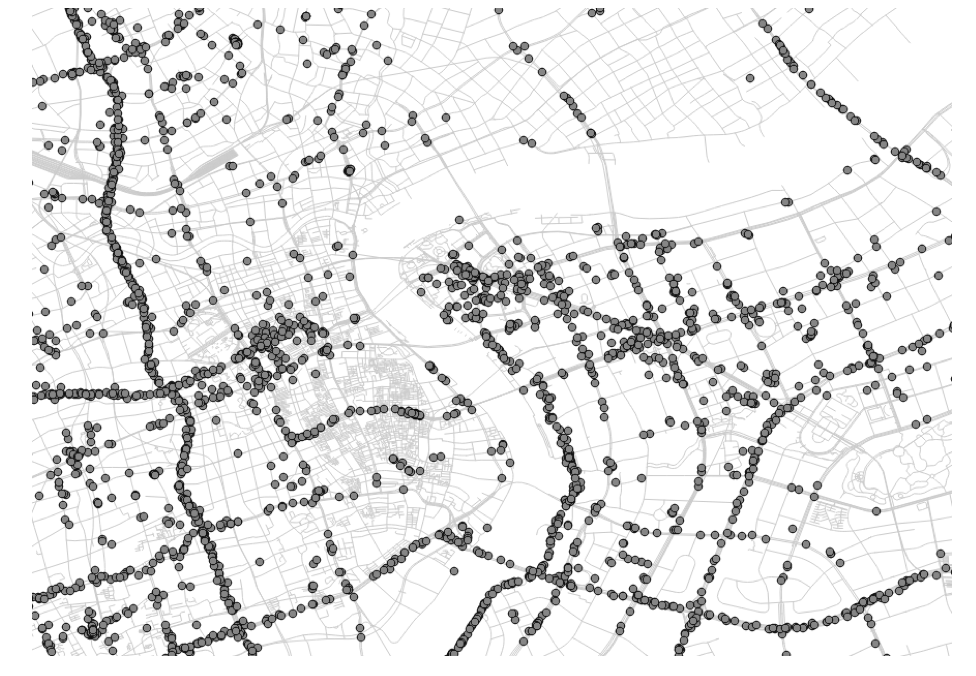
\includegraphics[width=0.5\textwidth]{chapter05/obd.png}
  \bicaption[fig:5-1]{上海私家车OBD数据样例}{上海私家车OBD数据样例}{Fig}{An example of Shanghai OBD private vehicle trajectories}
\end{figure}

\begin{table}[!htpb]
  	\centering
		\begin{tabular}{ |p{3cm}|p{4.5cm}|p{4.5cm}| }
		\hline
		 & 单机配置 & 集群配置(主机从机一致) \\
		 \hline
		 内存大小 & 4GB & 1GB \\
		 \hline
		 处理器 & 2.6GHz Intel Core i5 & 2.6GHz Intel Core i5 \\
		 \hline 
		 操作系统平台 & Mac OS X 10.11.6 & Ubuntu14.04 \\
		 \hline 
		\end{tabular}
	\bicaption[tab:5-1]{实验环境参数}{实验环境参数}{Table}{Environment of Experiment}
\end{table}


